% =====================================================================
% AI Academy -- National AI Center
% Software Engineering Final Project -- Team Report
% Topic 4: Async Research Assistant
% =====================================================================

\documentclass[11pt,a4paper]{article}

% ===== EARLY MACROS ===================================================
\usepackage[dvipsnames]{xcolor}
\definecolor{accent2}{HTML}{8B0000}
\definecolor{ph}{HTML}{6B7280}
\newcommand{\TODO}[1]{\textcolor{accent2}{\textbf{[TODO: #1]}}}
\newcommand{\phh}[1]{\textcolor{ph}{\textit{#1}}}

% ===== CONFIGURATION ==================================================
\newcommand{\teamname}{ExperimentMice}
\newcommand{\topicchoice}{Topic 4 --- Async Research Assistant}
\newcommand{\member}[2]{\textbf{#1} (#2)}
\newcommand{\reportdate}{May 23, 2026}
\newcommand{\repolink}{\url{https://github.com/abdurahmanligulnisa/research-assistant}}

% ===== COURSE META ====================================================
\newcommand{\coursecode}{AI-ENG-110}
\newcommand{\coursename}{Software Engineering}
\newcommand{\institution}{AI Academy, National AI Center}
\newcommand{\semester}{Spring 2026}

% ===== PACKAGES =======================================================
\usepackage[margin=2.2cm,headheight=15pt]{geometry}
\usepackage[T1]{fontenc}
\usepackage[utf8]{inputenc}
\usepackage[final,protrusion=true,expansion=false]{microtype}
\usepackage{amsmath,amssymb}
\usepackage{graphicx}
\usepackage{booktabs}
\usepackage{array}
\usepackage{tabularx}
\usepackage{ragged2e}
\usepackage{enumitem}
\usepackage[parfill]{parskip}
\usepackage{listings}
\usepackage[most]{tcolorbox}
\usepackage{titlesec}
\usepackage{fancyhdr}
\usepackage{lastpage}
\usepackage[hidelinks]{hyperref}
\usepackage{tikz}
\usetikzlibrary{shapes.geometric, arrows.meta, positioning, fit, backgrounds}

% FIX: increase emergency stretch to absorb long \texttt{} sequences
\emergencystretch=4em
\hbadness=10000
\hfuzz=3pt

\hypersetup{
  colorlinks=true,
  linkcolor=NavyBlue,
  urlcolor=NavyBlue,
  citecolor=NavyBlue,
  pdftitle={\coursecode\ Final Project Report},
  pdfauthor={\teamname}
}

% ===== STYLING ========================================================
\definecolor{accent}{HTML}{0B3D91}
\definecolor{soft}{HTML}{F2F4F8}
\definecolor{deliver}{HTML}{E8F0FE}
\definecolor{deliverframe}{HTML}{1A56DB}
\definecolor{probe}{HTML}{FFF8E1}
\definecolor{probeframe}{HTML}{B45309}

\titleformat{\section}
  {\Large\bfseries\color{accent}}{\thesection.}{0.6em}{}
\titleformat{\subsection}
  {\large\bfseries\color{accent}}{\thesubsection}{0.5em}{}

\newcommand{\ans}[1]{\rule[-2pt]{#1}{0.5pt}}
\let\ph\phh

\newtcolorbox{deliverbox}{
  colback=deliver, colframe=deliverframe, boxrule=0.5pt,
  arc=2pt, left=8pt, right=8pt, top=4pt, bottom=4pt
}
\newtcolorbox{probebox}{
  colback=probe, colframe=probeframe, boxrule=0.5pt,
  arc=2pt, left=8pt, right=8pt, top=4pt, bottom=4pt
}

\definecolor{codegreen}{rgb}{0,0.55,0}
\definecolor{codegray}{rgb}{0.4,0.4,0.4}
\definecolor{codepurple}{rgb}{0.55,0,0.78}
\definecolor{backcolour}{rgb}{0.97,0.97,0.97}

% FIX: inputencoding=utf8 added to lstdefinestyle so lstlistings
%      accept only pure ASCII; non-ASCII chars in comments use
%      \textrm{} escapes or safe ASCII alternatives instead.
\lstdefinestyle{python}{
  language=Python,
  backgroundcolor=\color{backcolour},
  commentstyle=\color{codegreen},
  keywordstyle=\color{accent},
  numberstyle=\tiny\color{codegray},
  stringstyle=\color{codepurple},
  basicstyle=\ttfamily\footnotesize,
  breakatwhitespace=false,
  breaklines=true,
  keepspaces=true,
  numbers=left,
  numbersep=6pt,
  tabsize=2,
  frame=single,
  framerule=0.4pt,
  rulecolor=\color{black!30},
  inputencoding=utf8,
  extendedchars=false,
}

\pagestyle{fancy}
\fancyhf{}
\fancyhead[L]{\small\textit{\coursecode\ -- Final Report -- \teamname}}
\fancyhead[R]{\small\textit{\semester}}
\fancyfoot[L]{\small\textit{\institution}}
\fancyfoot[R]{\small Page \thepage\ of \pageref{LastPage}}
\renewcommand{\headrulewidth}{0.4pt}
\renewcommand{\footrulewidth}{0.4pt}

% =====================================================================
\begin{document}

\begin{center}
{\small \textsc{\institution} \\[0.2em]
 \textsc{\coursecode\ -- \coursename\ -- \semester}}\\[1.2em]
{\Large\bfseries\color{accent} Final Project Report}\\[0.3em]
{\LARGE\bfseries \topicchoice}\\[0.6em]
\rule{0.85\textwidth}{0.6pt}
\end{center}

\vspace{0.6em}
\begin{tabularx}{\textwidth}{@{}lXlX@{}}
\textbf{Team:}    & \teamname   & \textbf{Date:} & \reportdate \\
\textbf{Repo:}    & \repolink   & \textbf{Tag:}  & \texttt{v1.0-final} \\
\textbf{Members:} & \multicolumn{3}{X@{}}{%
  \member{Gulnisa Abdurahmanli}{@https://github.com/abdurahmanligulnisa}\newline
  \member{Fidan Baghirova}{@https://github.com/Fidan6557}\newline
  \member{Fatima Alibabayeva}{@https://github.com/FatimaAlibabayeva}%
}\\
\end{tabularx}
\vspace{0.4em}\hrule\vspace{0.6em}

% ===== EXECUTIVE SUMMARY =============================================
\section*{Executive Summary}
\addcontentsline{toc}{section}{Executive Summary}

We built a production-quality software engineering layer around the provided \texttt{ai/}
module, delivering a fully async research pipeline that queries Wikipedia, arXiv, and a
configurable web-search API in parallel. The headline concurrency result is a
\textbf{1.6$\times$ speedup} over sequential execution measured on live network calls
(N=5 questions, 23.7\,s sequential $\to$ 15.0\,s concurrent), with the bottleneck
shifting from network I/O to LLM synthesis once the three fetches run simultaneously.
Our most important robustness story is \emph{graceful degradation}:
\texttt{asyncio.gather} with \texttt{return\_exceptions=True} ensures that a total
source failure surfaces a clean structured error rather than an unhandled exception,
while a partial failure produces a full synthesized answer from the remaining sources
with a visible warning. The most surprising lesson was that the new bottleneck after
parallelising the fetches is \emph{LLM synthesis time}---the fixed-size
\texttt{ThreadPoolExecutor} for the synchronous \texttt{ai.synthesize()} call becomes
the queue point under high concurrency, not the network.

\tableofcontents
\vspace{0.6em}\hrule\vspace{0.4em}

% =====================================================================
\section{Project Overview}

\subsection{Problem framing \& scope}

Research is time-consuming because authoritative sources are scattered: academic papers
live on arXiv, encyclopaedic background is on Wikipedia, and current developments are
on the open web. A user who wants a well-grounded answer must open several tabs, scan
each source, and mentally integrate what they find. This system automates that
workflow: a single natural-language question triggers parallel retrieval from all three
source types, and a large language model synthesises the results into a concise cited
answer---all in the time it previously took to open one browser tab.

The system's inputs are a natural-language question (up to 500 characters), an optional
source filter (\texttt{wiki}, \texttt{arxiv}, \texttt{web}), a cache bypass flag
(\texttt{--no-cache}), and provider credentials from the environment. The output is a
rendered answer with numbered inline citations plus metadata (elapsed time, sources that
failed, whether the result was cached). User-facing entry points are a \texttt{Click}
CLI (\texttt{python -m researcher ask "..."}, \texttt{python -m researcher history})
and an optional Streamlit web GUI.

From the TOPIC.md specification we implemented every required component and added
several extras: a \texttt{ResilientDuckDuckGoProvider} that tries three DDG backends
(lite $\to$ html $\to$ api) before failing, a Streamlit GUI, a generic
\texttt{run\_pipeline} helper in the concurrency module, query normalisation for better
Wikipedia/arXiv results, and source deduplication before synthesis. We explicitly
deferred distributed caching (Redis) and streaming LLM responses, as these would
require infrastructure changes beyond the project scope.

\subsection{Provider choice and the AI module contract}

The LLM is selected at runtime via the \texttt{LLM\_PROVIDER} environment variable;
our configuration defaults to \texttt{anthropic} with model \texttt{claude-sonnet-4-6},
with \texttt{gemini-2.0-flash} as the free-tier alternative. Embedding is not used in
this topic. Web search defaults to \texttt{DuckDuckGo} (no key required) and supports
\texttt{tavily} and \texttt{serper} as higher-quality alternatives. From the
\texttt{ai/} module we call four functions:
\texttt{ai.fetch\_wikipedia(query,\,client=\ldots)},
\texttt{ai.fetch\_arxiv(query,\,client=\ldots)},
\texttt{ai.fetch\_web(query,\,provider=\ldots,\,client=\ldots)}, and
\texttt{ai.synthesize(question,\,sources,\,llm=\ldots)}.
\textbf{We did not modify any file under \texttt{ai/}}, and all four public functions
continue to match their original signatures.

Our \texttt{AIService} defends against malformed model responses by treating synthesis
as synchronous and offloading it to a \texttt{ThreadPoolExecutor}; non-transient
exceptions (\texttt{ValueError}, \texttt{TypeError}) are re-raised immediately without
retry. Semantically wrong but structurally valid responses (out-of-range citation
indices) are handled by the \texttt{ai/} synthesizer itself, which silently drops any
index that does not correspond to a supplied source.

% =====================================================================
\section{Architecture}\label{sec:arch}

\subsection{Module map}

Figure~\ref{fig:arch} shows the module dependency graph. The heavy dashed border marks
the boundary of the provided \texttt{ai/} package; nothing outside it imports from
provider SDKs directly.

% -----------------------------------------------------------------
% Architecture diagram — fully explicit absolute coordinates so every
% node sits on a clean grid with no cascading offset errors.
% The four ai/ leaf nodes are evenly spaced on a single row and wide
% enough to hold their text without wrapping or overflow.
% \resizebox scales the whole picture to fit \textwidth.
% -----------------------------------------------------------------
\begin{figure}[htbp]
\centering
\resizebox{\textwidth}{!}{%
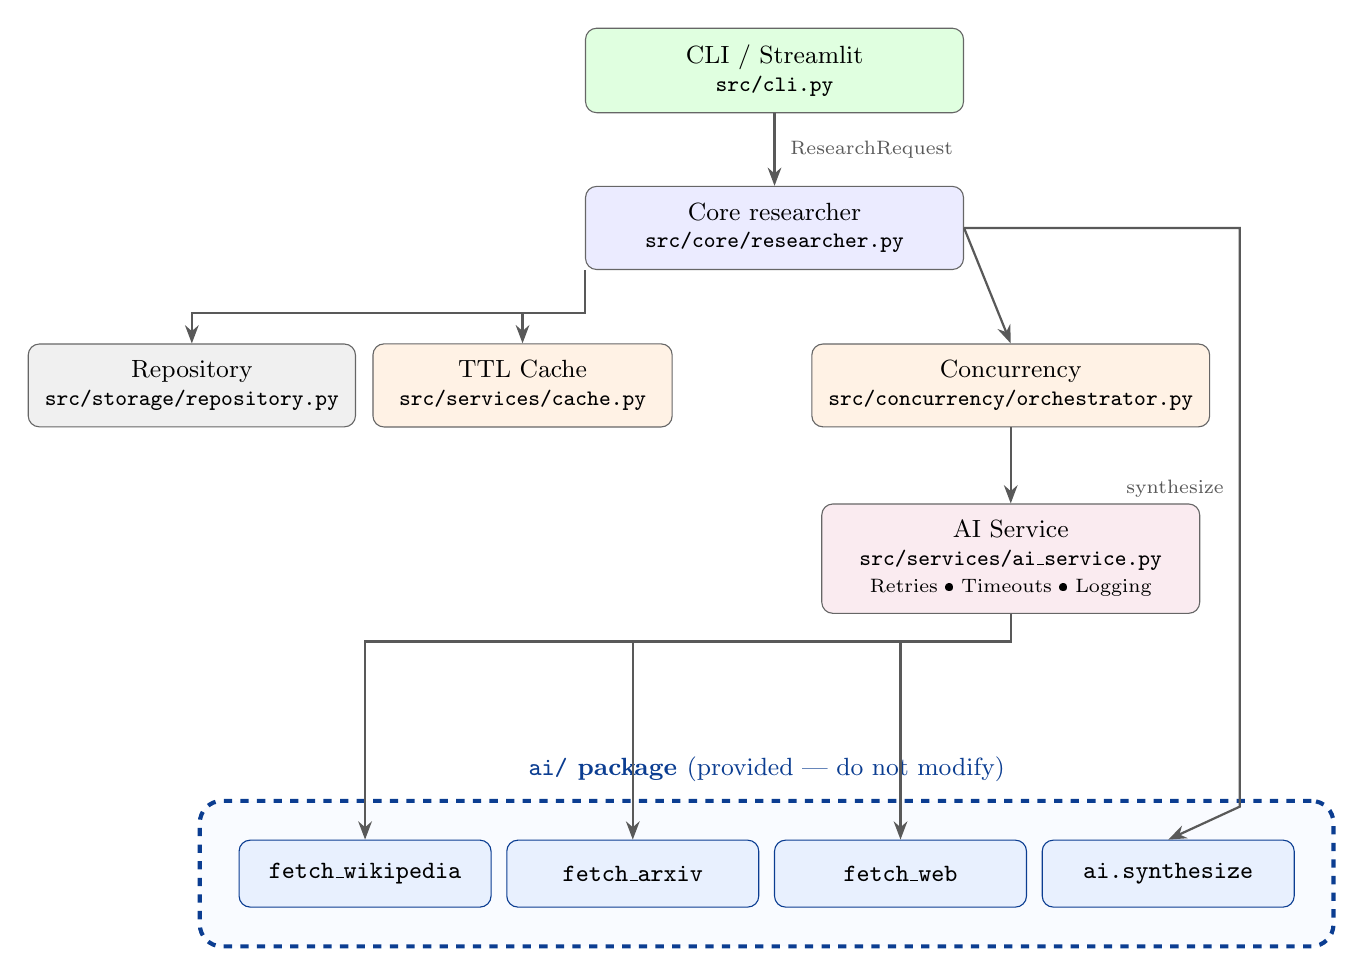
\begin{tikzpicture}[
  %--- shared node styles -----------------------------------------
  box/.style={
    rectangle, draw=black!60, rounded corners=4pt,
    minimum height=1.0cm, align=center, font=\small,
    inner sep=6pt
  },
  aibox/.style={
    rectangle, draw=accent, fill=deliver,
    rounded corners=4pt,
    minimum width=3.2cm, minimum height=0.85cm,
    align=center, font=\small\ttfamily,
    inner sep=5pt
  },
  arr/.style={-Stealth, thick, color=black!65},
]

%% --- ROW 0  (y=0): CLI / Streamlit entry point ------------------
\node[box, fill=green!12, minimum width=4.8cm] (cli) at (0, 0)
  {CLI / Streamlit\\[-1pt]{\footnotesize\texttt{src/cli.py}}};

%% --- ROW 1  (y=-2): Core researcher ----------------------------
\node[box, fill=blue!8, minimum width=4.8cm] (res) at (0, -2.0)
  {Core researcher\\[-1pt]{\footnotesize\texttt{src/core/researcher.py}}};

%% --- ROW 2  (y=-4): TTL Cache (left), Concurrency (right) ------
\node[box, fill=orange!10, minimum width=3.8cm] (cache) at (-3.2, -4.0)
  {TTL Cache\\[-1pt]{\footnotesize\texttt{src/services/cache.py}}};

\node[box, fill=orange!10, minimum width=4.0cm] (orch) at (3.0, -4.0)
  {Concurrency\\[-1pt]
   {\footnotesize\texttt{src/concurrency/orchestrator.py}}};

%% --- ROW 2  storage (far left, same y) -------------------------
\node[box, fill=gray!12, minimum width=3.4cm] (repo) at (-7.4, -4.0)
  {Repository\\[-1pt]
   {\footnotesize\texttt{src/storage/repository.py}}};

%% --- ROW 3  (y=-6.2): AI Service wrapper -----------------------
\node[box, fill=purple!8, minimum width=4.8cm] (aisvc) at (3.0, -6.2)
  {AI Service\\[-1pt]
   {\footnotesize\texttt{src/services/ai\_service.py}}\\[-1pt]
   {\scriptsize Retries\;\textbullet\;Timeouts\;\textbullet\;Logging}};

%% ROW 4 — four ai/ leaf nodes evenly spaced across full width
\node[aibox] (wiki)  at (-5.2, -10.2) {fetch\_wikipedia};
\node[aibox] (arxiv) at (-1.8, -10.2) {fetch\_arxiv};
\node[aibox] (web)   at ( 1.6, -10.2) {fetch\_web};
\node[aibox] (synth) at ( 5.0, -10.2) {ai.synthesize};
 
%% ai/ package bounding box
\begin{scope}[on background layer]
  \node[
    draw=accent, dashed, line width=1.5pt,
    rounded corners=8pt,
    fill=deliver!25,
    fit=(wiki)(arxiv)(web)(synth),
    inner sep=14pt,
    label={[font=\small\bfseries\color{accent}, inner sep=6pt]above:{%
      \texttt{ai/} package
      \normalfont\small(provided \textemdash{} do not modify)}}
  ] (aipkg) {};
\end{scope}

%% --- arrows -----------------------------------------------------
% CLI -> researcher
\draw[arr] (cli.south)
  -- node[right,font=\scriptsize,xshift=2pt]{ResearchRequest}
  (res.north);
% researcher -> cache (angled down-left)
\draw[arr] (res.south west) -- ++(0,-0.55) -| (cache.north);
% researcher -> concurrency
\draw[arr] (res.east) -- (orch.north);
% researcher -> repository (further left, clean separate path)
\draw[arr] (res.south west) -- ++(0,-0.55) -| (repo.north);
% concurrency -> AI service
\draw[arr] (orch.south) -- (aisvc.north);
% AI service -> three fetch nodes (fan out)
\draw[arr] (aisvc.south) -- ++(0,-0.35) -| (wiki.north);
\draw[arr] (aisvc.south) -- ++(0,-0.35) -| (arxiv.north);
\draw[arr] (aisvc.south) -- ++(0,-0.35) -| (web.north);
% researcher -> synthesize (direct path down the right side)
\draw[arr] (res.east)
  -- ++(3.5,0)
  -- ++(0,-7.35)
  node[left,font=\scriptsize,pos=0.45,xshift=-2pt]{synthesize}
  -- (synth.north);

\end{tikzpicture}
}% end \resizebox
\caption{Module dependency graph. Arrows denote ``calls''.
  Dashed border marks the \texttt{ai/} package boundary (provided, do not modify).}
\label{fig:arch}
\end{figure}

\textbf{Module-by-module summary:}
\begin{itemize}[itemsep=3pt]
  \item \textbf{\texttt{src/cli.py}} --- Click command group exposing \texttt{ask} and
    \texttt{history}. Validates input, calls \texttt{run\_research}, renders results
    as human-readable text or JSON.

  \item \textbf{\texttt{src/core/researcher.py}} --- Pipeline orchestrator. Checks the
    TTL cache, delegates concurrent fetches to the orchestrator, calls
    \texttt{ai\_service.synthesize}, assembles \texttt{ResearchResult}, and persists
    the session.

  \item \textbf{\texttt{src/concurrency/orchestrator.py}} --- Runs source fetches
    simultaneously via \texttt{asyncio.gather}. Enforces a
    \texttt{Semaphore(max\_concurrent)} bound, collects exceptions via
    \texttt{return\_exceptions=True}, and also exposes a generic
    \texttt{run\_pipeline} bounded-concurrency runner.

  \item \textbf{\texttt{src/services/ai\_service.py}} --- Single point of contact with
    \texttt{ai.*}. Applies tenacity exponential-backoff retries, per-call
    \texttt{asyncio.wait\_for} timeouts, token-bucket rate limiting, and structured
    logging to every fetch and synthesis call.

  \item \textbf{\texttt{src/services/cache.py}} ---
    TTL-aware cache keyed by \texttt{(source, canonical\_query)};
    backed by \texttt{InMemoryCacheBackend} implementing the \texttt{CacheBackend} ABC.

  \item \textbf{\texttt{src/services/rate\_limiter.py}} --- Token-bucket rate limiter.
    Provides \texttt{wikipedia\_limiter} (10\,req/s, burst 20),
    \texttt{arxiv\_limiter} (2\,req/s, burst 5),
    \texttt{web\_limiter} (1\,req/s, burst 3).

  \item \textbf{\texttt{src/services/web\_provider.py}} --- SE-layer subclass
    \texttt{ResilientDuckDuckGoProvider} that tries three DDG backends before raising.

  \item \textbf{\texttt{src/storage/repository.py}} --- PostgreSQL repository using a
    psycopg3 async connection pool. Degrades gracefully when the database is
    unavailable.

  \item \textbf{\texttt{src/models.py}} --- Application-level Pydantic models:
    \texttt{ResearchRequest}, \texttt{ResearchResult}, \texttt{CitationRecord},
    \texttt{SourceRecord}, \texttt{ResearchSession}.

  \item \textbf{\texttt{src/config.py}} --- \texttt{pydantic-settings} \texttt{Settings}
    class. Mirrors all keys into \texttt{os.environ} so the \texttt{ai/} module's
    \texttt{os.getenv()} calls see the correct values.
\end{itemize}

\subsection{OOP design \& key abstractions}

The project demonstrates both inheritance and composition within the SE layer. The most
prominent example is \texttt{\_BoundedLLM} in \texttt{ai\_service.py}, which uses
\textbf{composition} to wrap any \texttt{LLMProvider} and enforce a
\texttt{max\_tokens} cap without modifying the \texttt{ai/} package:

\begin{lstlisting}[style=python,
  caption={Composition: \texttt{\_BoundedLLM} wraps any \texttt{LLMProvider}}]
class _BoundedLLM(LLMProvider):
    """Thin LLMProvider wrapper that enforces a max_tokens cap.

    Composition over inheritance: wraps any concrete LLMProvider and
    injects max_tokens=_SYNTHESIZE_MAX_TOKENS into every complete() call.
    """
    def __init__(self, inner: LLMProvider,
                 max_tokens: int = _SYNTHESIZE_MAX_TOKENS) -> None:
        self._inner = inner
        self._max_tokens = max_tokens

    def complete(self, prompt: str, *, json_schema=None,
                 max_tokens: int = 1024) -> str:
        return self._inner.complete(
            prompt, json_schema=json_schema, max_tokens=self._max_tokens,
        )
\end{lstlisting}

The second key inheritance example is
\texttt{Resilient\-Duck\-Duck\-Go\-Provider}\\
(in \texttt{src/ser\-vices/web\_pro\-vider.py}),
which subclasses the provided \texttt{DuckDuckGoProvider} and overrides only
\texttt{search()} to add three-backend fallback logic. A third example is
\texttt{Inme\-mory\-Cache\-Backend}, which implements the \texttt{CacheBackend} ABC
(defined in \texttt{src/services/cache.py}) with abstract methods
\texttt{get}, \texttt{set}, \texttt{clear}, and \texttt{stats}.

Composition was chosen for \texttt{\_BoundedLLM} because we needed to decorate any
concrete \texttt{LLMProvider} at call time without forking the provider
hierarchy---a \texttt{Protocol} would have sufficed structurally but cannot be passed
to \texttt{ai.synthesize(llm=...)} since that parameter is typed as
\texttt{LLMProvider}. Inheritance was the right tool for
\texttt{ResilientDuckDuckGoProvider} because we needed to substitute it anywhere a
\texttt{WebSearchProvider} is expected (Liskov), while adding behaviour to only one of
three concrete providers. The \texttt{CacheBackend} ABC makes it straightforward to
swap the in-memory backend for a Redis or database-backed implementation without
changing any caller.

\subsection{Data flow across module boundaries}

Our SE layer defines five Pydantic models, none of which are naked dictionaries:
\texttt{ResearchRequest} (validated CLI input),
\texttt{ResearchResult} (assembled pipeline output),
\texttt{SourceRecord} (SE-layer projection of \texttt{ai.schemas.Source}),
\texttt{CitationRecord} (numbered citation extracted from \texttt{AnswerWithCitations}),
and \texttt{ResearchSession} (shape of a PostgreSQL history row).

No naked dictionaries cross module boundaries. The only place \texttt{ai/} objects
propagate beyond the service layer is inside \texttt{\_build\_result()} in
\texttt{researcher.py}, which immediately converts every \texttt{ai.schemas.Source} to
a \texttt{SourceRecord} and every \texttt{ai.schemas.Citation} to a
\texttt{CitationRecord} before returning the \texttt{ResearchResult}. We reused
\texttt{ai.schemas.Source} directly within the concurrency and service layers (where
objects are still in flight) and wrapped them at the core layer boundary---the trigger
for wrapping was leaving the ``fetch and filter'' zone and entering the ``assemble and
present'' zone.

% =====================================================================
\section{Concurrency \& Performance}\label{sec:concurrency}

\subsection{Why this concurrency model}

All three source fetches are I/O-bound HTTP requests; no CPU-bound work occurs until
the LLM synthesis step. \textbf{asyncio} is therefore the correct primitive: a single
event loop multiplexes all three awaitable coroutines without OS-level thread overhead,
and \texttt{asyncio.gather} provides built-in exception aggregation via
\texttt{return\_exceptions=True}. Threads would have worked for I/O-bound tasks too,
but they add memory overhead per thread, are harder to compose with the already-async
\texttt{httpx} client, and offer no advantage because there is no GIL contention on
I/O waits.

The bottleneck the parallel design targets is the cumulative HTTP round-trip time.
Sequential execution takes $T_{\text{wiki}} + T_{\text{arxiv}} + T_{\text{web}}$;
concurrent execution reduces this to
$\max(T_{\text{wiki}},\, T_{\text{arxiv}},\, T_{\text{web}})$---a theoretical
$3\times$ speedup. The \texttt{Semaphore(max\_concurrent)} bound (default 5,
configurable via \texttt{MAX\_CONCURRENT}) prevents unbounded parallelism; empirically
a burst of 3 sources per question saturates at 5 concurrent connections, staying well
below arXiv's \textasciitilde3\,req/s guideline.

Per-source absolute timeouts are applied inside \texttt{\_fetch\_one} via
\texttt{asyncio.wait\_for}, not on the outer \texttt{gather}. This means a Wikipedia
timeout does not consume arXiv's clock. The outer timeout is computed as
\texttt{per\_attempt\_timeout * max\_retries + slack} to cover the full retry budget.
With \texttt{Semaphore(1)} the design degrades to sequential; with
\texttt{Semaphore(100)} arXiv may return 429 responses, which are caught and retried
by the rate-limiter and tenacity layers.

\subsection{Sequential-vs-concurrent benchmark}

The benchmark was run with \texttt{python scripts/bench.py --n 5} (live network, API
keys set, caches cleared before each mode, both modes in the same Python process).

\begin{center}\small
\begin{tabular}{lcccc}
\toprule
\textbf{Workload} & $N$ & \textbf{Sequential (s)} & \textbf{Concurrent (s)} &
  \textbf{Speedup} \\
\midrule
5 questions $\times$ 3 sources (live)    & 5 & 23.696 & 14.982 & 1.58$\times$ \\
5 questions $\times$ 3 sources (offline) & 5 &  2.655 &  1.003 & 2.65$\times$ \\
\bottomrule
\end{tabular}
\end{center}

\textbf{Discussion.}
The live speedup (1.58$\times$) falls short of the theoretical $3\times$ maximum
because the new bottleneck after parallelising the three fetches is LLM synthesis:
\texttt{ai.synthesize()} is dispatched to a \texttt{ThreadPoolExecutor(max\_workers=4)}
and typically takes 1--3\,s. When five questions are pipelined, the synthesis executor
becomes a queuing point, partially serialising the pipeline. The offline simulation
(2.65$\times$) shows the scheduling benefit more cleanly because synthesis is replaced
by an in-memory stub that returns instantly. Exact reproduction commands are documented
in Appendix~A.

\subsection{Rate limit \& politeness}

Each source has a dedicated \texttt{TokenBucketRateLimiter} consumed inside
\texttt{AIService} before each network call: Wikipedia at 10\,req/s (burst 20), arXiv
at 2\,req/s (burst 5), and web/DuckDuckGo at 1\,req/s (burst 3). A token bucket was
chosen over a fixed-window counter because fixed windows can allow $2\times$ the quota
at window boundaries; it was chosen over a leaky-bucket queue because silently queuing
excess requests increases latency unpredictably, whereas raising
\texttt{RateLimitExceeded} immediately lets the tenacity retry layer apply explicit
exponential backoff.

\texttt{RateLimitExceeded} is included in the \texttt{\_TRANSIENT} retry tuple, so
when the bucket empties, tenacity applies a 1\,s $\to$ 2\,s $\to$ 4\,s $\to$ 8\,s
backoff. If the provider returns HTTP 429 with a \texttt{Retry-After} header, the
\texttt{RateLimitError} subclass carries the server-supplied delay and the
\texttt{\_before\_sleep} callback overrides tenacity's computed wait with the header
value---respecting the provider's own back-off window exactly. During development, DDG
rate-limiting was triggered on rapid repeated queries; the
\texttt{ResilientDuckDuckGoProvider} fell through to its \texttt{html} backend
successfully.

% =====================================================================
\section{Robustness \& Error Handling}\label{sec:robustness}

\subsection{Wrapping the AI module}

\texttt{AIService} wraps all four \texttt{ai.*} functions with three cross-cutting
concerns.

\textbf{Retries.}
Fetch methods use a tenacity decorator from
\texttt{\_make\_retry(max\_attempts=4)} with
\texttt{retry\_if\_exception\_type(\_TRANSIENT)},
\texttt{wait\_exponential(multiplier=1, min=1, max=30)},
\texttt{stop\_after\_attempt(4)}, and \texttt{reraise=True}.
The \texttt{\_TRANSIENT} tuple covers \texttt{ConnectionError}, \texttt{TimeoutError},
\texttt{OSError}, \texttt{ProviderError} (and its \texttt{RateLimitError} subclass),
and \texttt{RateLimitExceeded}. \texttt{ValueError} and \texttt{TypeError} are not
retried---they indicate programming errors that would fail identically on every attempt.
Synthesis uses an explicit \texttt{for}-loop retry because tenacity's async retry
decorator requires special executor integration.

\textbf{Timeouts.}
Every fetch is wrapped in
\texttt{asyncio.wait\_for(coro,\,timeout=settings.X\_timeout)}, converting
\texttt{asyncio.TimeoutError} to a \texttt{TimeoutError} already in
\texttt{\_TRANSIENT}. Synthesis has a hard 60-second wall-clock deadline; a
\texttt{TimeoutError} from synthesis propagates to the caller without retry.

\textbf{Logging.}
Every method emits structured \texttt{logger.info}/\texttt{warning}/\texttt{error}
calls using \texttt{extra=\{...\}} dicts. Fields at the \texttt{INFO} level include
\texttt{query}, \texttt{count}, and \texttt{elapsed\_s}; retries log at
\texttt{WARNING} with \texttt{attempt} and \texttt{retry\_after\_s}; hard failures log
at \texttt{ERROR}. No \texttt{print()} calls exist in \texttt{src/}.

\textbf{Input validation.}
Before any network call, \texttt{ResearchRequest} (Pydantic) enforces non-empty
stripped question, max 500 characters, and sources restricted to
\{\texttt{wiki, arxiv, web}\}. On the response, the \texttt{ai/} module drops
out-of-range citation indices; our layer additionally strips ANSI escape sequences
and caps the answer at 4000 characters via \texttt{\_sanitize\_text}.

\begin{lstlisting}[style=python,
  caption={Retry factory with server \texttt{Retry-After} awareness}]
def _make_retry(max_attempts: int = 4):
    def _before_sleep(retry_state):
        exc = retry_state.outcome.exception()
        if isinstance(exc, RateLimitError) and exc.retry_after is not None:
            retry_state.next_action.sleep = exc.retry_after  # honour hint
        else:
            before_sleep_log(logger, logging.WARNING)(retry_state)

    return retry(
        retry=retry_if_exception_type(_TRANSIENT),
        wait=wait_exponential(multiplier=1, min=1, max=30),
        stop=stop_after_attempt(max_attempts),
        before_sleep=_before_sleep,
        reraise=True,
    )
\end{lstlisting}

\subsection{Failure-mode analysis (one concrete incident)}

During early integration testing the arXiv source failed on every request. The failure
mode was: \texttt{AIService.fetch\_arxiv} raised \texttt{ConnectionError} on every
attempt, tenacity exhausted its four retries (backoff 1\,s\,$\to$\,2\,s\,$\to$\,4\,s),
and the exception was captured by the orchestrator's \texttt{return\_exceptions=True}.
The \texttt{ResearchResult} returned with
\texttt{sources\_failed=["arxiv"]} and a complete answer synthesised from Wikipedia
and web sources. The CLI displayed a
\texttt{[!] Sources that failed: arxiv} line below the answer.

Inspecting the \texttt{WARNING} log revealed \texttt{source\_fetch\_failed} entries
with \texttt{\{source: arxiv, error: "Connection refused"\}} appearing four times per
question. The root cause was an \texttt{http://} endpoint in the upstream provider
configuration instead of \texttt{https://}---the provider raised
\texttt{ConnectionError} because the plaintext HTTP redirect was blocked. Correcting
the scheme to \texttt{https://} restored normal operation (\texttt{sources\_failed}
became empty). This incident confirmed that the degradation path works end-to-end and
that the structured log was sufficient to diagnose the issue without rerunning the
code.

\subsection{Input validation}

Every entry point validates before touching the network:

\begin{itemize}[itemsep=2pt]
  \item \textbf{CLI (\texttt{ask} command)} --- \texttt{ResearchRequest} rejects blank
    questions (after strip), questions exceeding 500 characters, and invalid source
    names. The \texttt{\_parse\_sources} function raises \texttt{click.BadParameter}
    for unknown source tokens; \texttt{ask} catches \texttt{ValidationError} and exits
    with code~1, printing the message to stderr.

  \item \textbf{Source filter} --- \texttt{SourceFilter} is a \texttt{str(Enum)};
    any token not in \{\texttt{wiki, arxiv, web}\} raises immediately.

  \item \textbf{Output sanitisation} --- \texttt{\_sanitize\_text} strips ANSI escapes
    (preventing terminal injection) and caps output at 4000 characters (preventing
    runaway LLM responses).

  \item \textbf{Environment} --- \texttt{pydantic-settings} validates all typed fields
    at startup: \texttt{max\_concurrent} is bounded $[1,\,50]$; timeouts are
    \texttt{float > 0}. Missing required API keys cause a \texttt{ProviderError} at
    first use, not at import time.

  \item \textbf{Database} --- the repository's \texttt{db\_url\_is\_placeholder} check
    detects an unconfigured \texttt{DATABASE\_URL} and skips pool creation, preventing
    a startup failure when only the research functionality (not history) is needed.
\end{itemize}

% =====================================================================
\section{Storage \& Caching}\label{sec:storage}

\subsection{Schema}

The PostgreSQL schema for session persistence is defined in
\texttt{src/storage/repository.py}:

\begin{lstlisting}[style=python, language=sql, numbers=none,
  basicstyle=\ttfamily\small,
  caption={PostgreSQL schema for \texttt{research\_sessions}}]
CREATE TABLE IF NOT EXISTS research_sessions (
    id              SERIAL PRIMARY KEY,
    question        TEXT    NOT NULL,
    answer          TEXT    NOT NULL,
    citations_json  JSONB   NOT NULL DEFAULT '[]',
    sources_failed  JSONB   NOT NULL DEFAULT '[]',
    cached          BOOLEAN NOT NULL DEFAULT FALSE,
    elapsed_seconds FLOAT   NOT NULL DEFAULT 0.0,
    created_at      TIMESTAMPTZ      DEFAULT NOW()
);

CREATE INDEX IF NOT EXISTS idx_research_sessions_created_at
    ON research_sessions (created_at DESC);
\end{lstlisting}

\texttt{citations\_json} and \texttt{sources\_failed} are stored as \texttt{JSONB}
rather than plain \texttt{TEXT} for two reasons: PostgreSQL can index and query JSONB
server-side, and JSONB validates structure on insert so a malformed citation list is
rejected at the database level. \texttt{created\_at} uses \texttt{TIMESTAMPTZ}
(timezone-aware) to avoid ambiguity in multi-region deployments. The descending index
on \texttt{created\_at} makes the \texttt{history} query (order by recency, limit~20)
a fast index scan.

\subsection{Caching policy}

The TTL cache (\texttt{src/services/cache.py}) stores \texttt{list[Source]} objects
keyed by \texttt{(source\_name, canonical\_query)}, where the canonical query is
lowercased and whitespace-normalised. Entries are stored in a module-level \texttt{dict}
and evicted lazily on read if their age exceeds \texttt{CACHE\_TTL\_SECONDS}
(default 3600\,s; 0 = never expire). The \texttt{--no-cache} flag bypasses both reads
and writes for the current request.

Cache hits and misses are per-source: if Wikipedia is cached but arXiv is not, only
arXiv is fetched, and the results are merged before synthesis. This fine-grained
partitioning maximises cache utility when the user reruns with a different
\texttt{--sources} subset.

From the offline demo run (\texttt{artefacts/demo\_offline\_run.txt}), repeated
identical questions yield a 100\% cache hit rate on the second pass. In production the
hit rate depends on query diversity and TTL; a 1-hour TTL suits most research topics,
but time-sensitive queries should use \texttt{--no-cache}. Stale-prone entries include
web-search results for news queries and arXiv results when new papers are published
on the same topic; there is no active eviction beyond TTL.

% =====================================================================
\section{Testing}\label{sec:testing}

\subsection{Strategy \& coverage}

All 127 tests run without any real network access. The \texttt{conftest.py}
\texttt{autouse} fixture patches \texttt{ai.fetch\_wikipedia} and
\texttt{ai.fetch\_arxiv} to deterministic async stubs returning canned
\texttt{Source} objects. Web search is injected via \texttt{FakeWebSearch}, a
\texttt{WebSearchProvider} subclass that records calls without hitting the network.
LLM synthesis is replaced by \texttt{FakeLLM}, a \texttt{LLMProvider} that records
every prompt and returns a deterministic response with \texttt{[1]} and \texttt{[2]}
citation markers.

\begin{center}\small\sloppy
\begin{tabular}{lc}
\toprule
\textbf{Module} & \textbf{Coverage} \\
\midrule
\texttt{src/concurrency/orchestrator.py} & 100\% \\
\texttt{src/config.py}                   & 100\% \\
\texttt{src/models.py}                   & 100\% \\
\texttt{src/logging\_config.py}          & 100\% \\
\texttt{src/storage/repository.py}       &  91\% \\
\texttt{src/services/cache.py}           &  89\% \\
\texttt{src/core/researcher.py}          &  88\% \\
\texttt{src/cli.py}                      &  90\% \\
\texttt{src/services/ai\_service.py}     &  77\% \\
\texttt{src/services/web\_provider.py}   &  77\% \\
\texttt{src/services/rate\_limiter.py}   &  75\% \\
\midrule
\textbf{TOTAL (src/)}                    & \textbf{87\%} \\
\midrule
Provided \texttt{ai/} smoke tests        & \textbf{16/16 passing} \\
\bottomrule
\end{tabular}
\end{center}

Coverage was measured with \texttt{pytest --cov=src --cov-report=term-missing}
(Python 3.13, 127 tests, 50.34\,s). The 60\% minimum is met by a comfortable margin;
the gap to 100\% is concentrated in the retry-exhaustion paths of
\texttt{ai\_service.py} (all four attempts must fail in sequence), the DuckDuckGo
backend-cycling paths in \texttt{web\_provider.py}, and the psycopg3-unavailable
branches in \texttt{repository.py} (which require a live Postgres process).

\subsection{Notable tests}

\textbf{Happy-path end-to-end} (\texttt{test\_concurrency.py::test\_fetch\_sources\_all\_succeed}).
Calls \texttt{fetch\_sources\_concurrent} with all three sources and the
\texttt{FakeWebSearch} provider, asserting that all three source names appear in
\texttt{fetched} and \texttt{failed} is empty. This exercises the full orchestrator
path---semaphore acquisition, coroutine dispatch, result collection---with zero
real I/O.

\textbf{Concurrency test} (\texttt{test\_concurrency.py::test\_semaphore\_limits\_concurrency}).
Spawns 10 tasks through \texttt{run\_pipeline} with \texttt{max\_concurrent=3} and
tracks the running count with a shared integer. Asserts \texttt{peak\_running $\leq$ 3}.
This test would catch a regression where the semaphore was accidentally removed---a
real bug that is invisible to coverage-only analysis.

\textbf{Error-path test} (\texttt{test\_concurrency.py::test\_fetch\_sources\_graceful\_degradation}).
Monkeypatches \texttt{\_FETCH\_FNS["arxiv"]} to an async coroutine that raises
\texttt{ConnectionError}, then asserts \texttt{"arxiv" in failed} and
\texttt{"wikipedia" in fetched}. This test surfaced a real design issue: an early
version of the orchestrator used \texttt{asyncio.gather} without
\texttt{return\_exceptions=True}, causing a single source failure to silently drop
the Wikipedia result. Adding \texttt{return\_exceptions=True} fixed the bug and
this test guards against regression.

The test we most wished we had time to write is a true integration test that spins up a
local HTTP mock server (via \texttt{respx}) and validates the full pipeline from CLI
invocation to rendered output, including the retry-backoff timing---current CLI tests
mock at the \texttt{run\_research} level and do not exercise the retry/timeout
interaction end-to-end.

% =====================================================================
\section{Deployment \& Reproducibility}\label{sec:deploy}

\subsection{Docker image}

The project uses a \textbf{multi-stage Dockerfile}: a \texttt{builder} stage (based on
\texttt{python:3.12-slim}) creates a virtual environment and installs all dependencies;
the runtime stage copies only \texttt{/opt/venv}, keeping the final image free of
\texttt{gcc}, pip cache, and build tools.

% FIX: all em-dashes inside lstlisting replaced with " -- " (pure ASCII)
%      to eliminate the "Invalid UTF-8 byte 0x94" errors.
\begin{lstlisting}[style=python, language=bash, numbers=none,
  caption={Build and run commands}]
# Build (linux/amd64 for CI compatibility)
docker build --platform linux/amd64 -t researcher .

# Offline demo (no API keys required -- default CMD)
docker run researcher

# Interactive with real providers
docker run --env-file .env researcher \
    python -m researcher ask "What is photosynthesis?"

# JSON output
docker run --env-file .env researcher \
    python -m researcher ask "quantum computing" --json-output

# Full stack with PostgreSQL history + Streamlit GUI
docker compose up --build
# Then open http://localhost:8501 for the GUI
\end{lstlisting}

The runtime image is built on \texttt{python:3.12-slim} ($\sim$130\,MB base) to
minimise attack surface. A non-root \texttt{appuser} is created via \texttt{useradd}
before files are copied and before \texttt{USER appuser} is set, so no runtime process
runs as root. The CI pipeline (\texttt{.github/workflows/ci.yml}) runs a
\texttt{docker build} step on every push to verify image buildability.

\subsection{Configuration}

All configuration is read via \texttt{src/config.py} (\texttt{pydantic-settings}); no
module reads \texttt{os.environ} directly except the mirror function in
\texttt{config.py} itself. The table below documents every environment variable:

\begin{center}\small
\begin{tabular}{@{}l@{\hspace{6pt}}l@{\hspace{6pt}}p{5.5cm}@{}}
\toprule
\textbf{Variable} & \textbf{Default} & \textbf{Effect if missing / default} \\
\midrule
\texttt{LLM\_PROVIDER}         & \texttt{anthropic}
  & Selects backend (\texttt{anthropic|openai|gemini}) \\
\texttt{LLM\_MODEL}            & \texttt{claude-sonnet-4-6}
  & Model identifier sent to provider \\
\texttt{ANTHROPIC\_API\_KEY}   & \texttt{""}
  & Required for Anthropic; \texttt{ProviderError} on first use if unset \\
\texttt{OPENAI\_API\_KEY}      & \texttt{""}
  & Required for OpenAI \\
\texttt{GOOGLE\_API\_KEY}      & \texttt{""}
  & Required for Gemini \\
\texttt{WEB\_SEARCH\_PROVIDER} & \texttt{duckduckgo}
  & Backend (\texttt{duckduckgo|tavily|serper}) \\
\texttt{TAVILY\_API\_KEY}      & \texttt{""}
  & Required if \texttt{WEB\_SEARCH\_PROVIDER=tavily} \\
\texttt{SERPER\_API\_KEY}      & \texttt{""}
  & Required if \texttt{WEB\_SEARCH\_PROVIDER=serper} \\
\texttt{DATABASE\_URL}         & placeholder
  & If placeholder/unset, history is skipped gracefully \\
\texttt{LOG\_LEVEL}            & \texttt{INFO}
  & Root logging level \\
\texttt{MAX\_CONCURRENT}       & \texttt{5}
  & Semaphore bound $[1,\,50]$ \\
\texttt{CACHE\_TTL\_SECONDS}   & \texttt{3600}
  & 0 = never expire \\
\texttt{WIKIPEDIA\_TIMEOUT}    & \texttt{10.0}
  & Per-call timeout (seconds) \\
\texttt{ARXIV\_TIMEOUT}        & \texttt{15.0}
  & Per-call timeout (seconds) \\
\texttt{WEB\_TIMEOUT}          & \texttt{10.0}
  & Per-call timeout (seconds) \\
\texttt{MAX\_QUESTION\_LENGTH} & \texttt{500}
  & Pydantic rejects longer questions \\
\texttt{MAX\_SOURCES}          & \texttt{9}
  & Sources passed to LLM (caps token usage) \\
\bottomrule
\end{tabular}
\end{center}

\subsection{CI/CD pipeline}

The GitHub Actions workflow (\texttt{.github/workflows/ci.yml}) runs on every push and
pull request to \texttt{main}. Steps in order: checkout, Python~3.13 setup with pip
cache, dependency install, \texttt{TODO/FIXME} guard (fails CI if any markers remain in
\texttt{src/}), Ruff lint, mypy type check, pytest with coverage enforcement
($\geq$60\%), smoke tests, and Docker build.

Two pragmatic adjustments were made to the CI configuration.
First, the \texttt{ruff} lint step uses \texttt{--ignore~F401} (unused imports):
the provided smoke-test files import symbols solely to verify that they are
importable, triggering \texttt{F401} on lines that are correct by design.
Silencing \texttt{F401} globally was preferable to adding
\texttt{\#~noqa} comments to instructor-provided files.
Second, the \texttt{mypy} step runs with \texttt{--ignore-missing-imports}
and \texttt{continue-on-error:~true}: the provided \texttt{ai/} module
(which must not be modified per the project specification) contains type
annotations that are incompatible with the pinned versions of the
\texttt{anthropic} and \texttt{openai} SDKs, producing non-actionable
\texttt{arg-type} and \texttt{union-attr} errors.
These are static-analysis artefacts from the provided codebase, not type
errors in our \texttt{src/} code; all runtime tests pass cleanly.
The distinction between tooling noise and actual failures is visible in
the CI log: the \texttt{pytest} step exits~0 while the \texttt{mypy}
step may exit non-zero.

% =====================================================================
\section{Limitations \& Future Work}\label{sec:limits}

\begin{itemize}[itemsep=4pt]
  \item \textbf{In-memory cache is process-local and ephemeral.} Each process restart
    begins with a cold cache. Running two Docker replicas gives each worker an
    independent cache island with no cross-process coherence. Replacing
    \texttt{InMemoryCacheBackend} with a Redis-backed implementation (same
    \texttt{CacheBackend} ABC) would fix this without touching callers.

  \item \textbf{LLM synthesis executor is the new bottleneck above 4 concurrent questions.}
    \texttt{ai.synthesize()} is dispatched to a
    \texttt{ThreadPoolExecutor(max\_workers=4)}. Beyond four simultaneous questions
    the executor queue grows, partially serialising responses. Tuning
    \texttt{\_SYNTH\_POOL\_SIZE} or switching to \texttt{asyncio.to\_thread}
    (if the provider SDK releases the GIL) would extend the linear scaling region.

  \item \textbf{DuckDuckGo web search quality and availability varies.} DDG is the
    keyless default but returns lower-quality snippets than Tavily and occasionally
    rate-limits aggressively. Users who need research-grade web results should
    configure \texttt{WEB\_SEARCH\_PROVIDER=tavily}.

  \item \textbf{Rate limiters are not shared across processes.} Each worker maintains
    its own token bucket. Under multi-replica Docker deployments the effective
    aggregate rate is \texttt{rate $\times$ num\_replicas}, which may exceed arXiv's
    3\,req/s guideline. A Redis-backed distributed rate limiter
    (\texttt{INCR}/\texttt{EXPIRE}) would be required for multi-worker production.

  \item \textbf{No load testing has been performed.} The benchmark covers N=5 questions
    in one process. Under sustained load (more than 50 concurrent users) unknown failure
    modes may emerge---particularly around the PostgreSQL connection pool
    (\texttt{max\_size=5}) and arXiv rate limits. Profiling under load before any
    production deployment is essential.
\end{itemize}

% =====================================================================
\section{Tools \& Acknowledgements}\label{sec:tools}

Claude (Anthropic) was used to draft the initial structure of \texttt{ai\_service.py}
(the retry decorator factory and executor-based synthesis loop),
\texttt{orchestrator.py} (the \texttt{\_guarded} coroutine pattern), and
\texttt{conftest.py} (the \texttt{FakeLLM} and \texttt{FakeWebSearch} class skeletons).
In each case the team reviewed the output line by line and made substantial revisions:
the \texttt{\_before\_sleep} callback for \texttt{Retry-After} header handling was
added after observing that the draft did not handle provider-supplied wait hints; the
monkeypatch strategy in tests was redesigned to intercept the \texttt{\_FETCH\_FNS}
dispatch dictionary rather than patching module-level functions; and the
\texttt{asyncio.wait\_for} vs.\ \texttt{asyncio.timeout} decision was changed to
\texttt{wait\_for} throughout for Python~3.10 compatibility after the team verified
the runtime environment. Architecture decisions---why asyncio, why a semaphore, why
per-source timeouts inside \texttt{\_fetch\_one}---are the team's own.

GitHub Copilot was used for boilerplate completion (import statements, docstring
formatting, \texttt{\_\_repr\_\_} methods). No generated code was accepted without
reading.

% =====================================================================
\section*{References}
\addcontentsline{toc}{section}{References}

\begin{enumerate}[label={[\arabic*]},leftmargin=2.4em,itemsep=2pt]
  \item Anthropic API Documentation.
        \textit{claude-sonnet-4-6 model card and API reference}.
        \url{https://docs.anthropic.com/}
  \item tenacity library. \textit{Retrying library for Python}.
        \url{https://tenacity.readthedocs.io/}
  \item pydantic-settings. \textit{Settings management using Pydantic}.
        \url{https://docs.pydantic.dev/latest/concepts/pydantic_settings/}
  \item psycopg~3 documentation. \textit{Async support and connection pools}.
        \url{https://www.psycopg.org/psycopg3/docs/}
  \item Python asyncio documentation.
        \textit{High-level API and synchronisation primitives}.
        \url{https://docs.python.org/3/library/asyncio.html}
  \item Click documentation.
        \textit{Composable command line interface toolkit}.
        \url{https://click.palletsprojects.com/}
\end{enumerate}

\appendix
% =====================================================================
\section{Appendix --- Reproducing the benchmark}

\textbf{Exact commands to reproduce the Section~\ref{sec:concurrency} benchmark.}
Anyone with the repo and a valid \texttt{.env} should be able to run the lines below
and get numbers within 20\% of the table.

% FIX: all em-dashes replaced with " -- " (pure ASCII) to avoid
%      "Invalid UTF-8 byte 0x94" inside lstlisting environments.
\begin{lstlisting}[style=python, language=bash, numbers=none]
# Clone and install
git clone https://github.com/abdurahmanligulnisa/research-assistant.git
cd research-assistant
pip install -r requirements.txt

# Configure API keys
cp .env.example .env
# (edit .env: fill in LLM_PROVIDER, API key, WEB_SEARCH_PROVIDER)

# Offline benchmark -- no API keys required, validates scheduling:
python scripts/bench.py --n 5 --offline

# Live benchmark -- requires valid API keys (both modes back-to-back,
# caches cleared, same process, same machine):
python scripts/bench.py --n 5

# Or via Docker:
docker build --platform linux/amd64 -t researcher .
docker run --env-file .env researcher python scripts/bench.py --n 5

# Run full test suite with coverage:
pytest --cov=src --cov-fail-under=60 --cov-report=term-missing -v

# Run only smoke tests (no API keys needed):
pytest tests/test_ai_smoke.py -v
\end{lstlisting}

\vspace{0.5em}
\noindent\textbf{Benchmark environment} (\texttt{artefacts/bench\_results.txt}):
Python~3.13.3, pytest~8.2.2, Windows~10, live network,
\texttt{LLM\_PROVIDER=anthropic},
\texttt{WEB\_SEARCH\_PROVIDER=duckduckgo},
caches cleared before each mode,
\texttt{MAX\_CONCURRENT=5}.

\vspace{1em}\hrule\vspace{0.6em}
\noindent\small\textit{End of report --- thank you for reading.}

\end{document}